\message{ !name(latex.tex)}\documentclass[a4paper,10pt]{book}
\usepackage[english]{babel}     
\usepackage[utf8]{inputenc}     % accent symbols
\usepackage[T1]{fontenc}
\usepackage{lmodern}
\usepackage{microtype}
\usepackage{natbib}
\usepackage{tocbibind}          
\usepackage{amsmath}            % math symbols
\usepackage{amsthm}             % math symbols
\usepackage[colorlinks=true,linkcolor=red]{hyperref} % hyper link

% for code
\usepackage{listings}
\usepackage{color,xcolor}
\definecolor{mygreen}{rgb}{0,0.6,0}
\definecolor{mygray}{rgb}{0.9,0.9,0.9}
\definecolor{mymauve}{rgb}{0.58,0,0.82}
\lstset{
backgroundcolor=\color{mygray},
numbers=left,                    
columns=fullflexible,
breaklines=true,      
captionpos=b,         
tabsize=4,            
commentstyle=\color{mygreen}, 
escapeinside={\%*}{*)},       
keywordstyle=\color{blue},    
% stringstyle=\color{mymauve}\monaco,
frame=single,                        
rulesepcolor=\color{red!20!green!20!blue!20},
% identifierstyle=\color{red},
%% language=c++,
basicstyle=\tiny
}

\usepackage{indentfirst}
\setlength{\parindent}{2em}
\usepackage[onehalfspacing]{setspace}
% graph
\usepackage{pdfpages}
\usepackage{graphicx}
% box
\usepackage{booktabs}
\usepackage{tcolorbox}

%% user defined command
\newcommand{\keyword}[1]{\textbf{#1}}
\newcommand{\keywords}[1]{\textbf{#1}}
\newcommand{\lcmd}[1]{\texttt{#1}}
\newcommand{\head}[1]{\textnormal{\textbf{#1}}}
\newcommand{\itwords}[1]{\textit{#1}}

\usepackage{float}
% all symbols
\usepackage{tipa}
\usepackage{tipx}

\usepackage{datetime}
% \usepackage{movie15}


% variable
% TODO
\newcommand{\pdfauthor}{李明明}
\newcommand{\pdftitle}{工作}
\newcommand{\pdfsubject}{工作中的经验与教训}
\newcommand{\pdfkeywords}{工作经验与教训}
\newcommand{\bookname}{工作收获}
\newcommand{\bookoneword}{工作中吸取的经验和教训}
\newcommand{\timeandcompany}{2020年12月1日}

\usepackage{bm}
\usepackage{amsfonts}
\begin{document}

\message{ !name(mytikz.tex) !offset(10) }

We are working on
\begin{tikzpicture}
  \draw (-1.5,0) -- (1.5,0);
  \draw (0,-1.5) -- (0,1.5);
\end{tikzpicture}.
\end{document}
\end{lstlisting}



We are working on
\begin{tikzpicture}
  \draw (-1.5,0) -- (1.5,0);
  \draw (0,-1.5) -- (0,1.5);
\end{tikzpicture}.



\begin{lstlisting}
\tikz \draw (-1.5,0) -- (1.5,0) -- (0,-1.5) -- (0,1.5);
\end{lstlisting}

\tikz \draw (-1.5,0) -- (1.5,0) -- (0,-1.5) -- (0,1.5);

\keyword{\textbackslash{}tikz} either takes one argument (starting with an opening braces) or collects everything up to the next semicolon and puts it inside a \keyword{tikzpicture} endironment.




\subsection{Straight path}
\label{sec:straight-path}

\begin{lstlisting}
\draw (0,0) -- (1.5,0);
\end{lstlisting}

\begin{tikzpicture}
  \draw (0,0) -- (1.5,0);
\end{tikzpicture}

The coordinates are used to locate the positions and \keyword{--} is used for drawing.

\subsection{Curved path}
\label{sec:curved-path}

\begin{lstlisting}
 \filldraw [gray] (0,0) circle (2pt)
                   (1,1) circle (2pt)
                   (2,1) circle (2pt)
                   (2,0) circle (2pt);
  \draw (0,0) .. controls (1,1) and (2,1) .. (2,0);
\end{lstlisting}


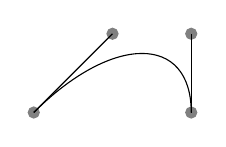
\begin{tikzpicture}
  \filldraw [gray] (0,0) circle (2pt)
  (1,1) circle (2pt)
  (2,1) circle (2pt)
  (2,0) circle (2pt);
  \draw (0,0) .. controls (1,1) and (2,1) .. (2,0);
  \draw (0,0) -- (1,1);
  \draw (2,1) -- (2,0);
\end{tikzpicture}

You can leave out the \keyword{and} (second control point), which causes the first one to be used twice.



\subsection{Circle path}
\label{sec:circle-path}

\begin{lstlisting}
\draw (0,0) circle (10pt);
\end{lstlisting}


\begin{tikzpicture}
  \draw (0,0) circle (10pt);
\end{tikzpicture}



\begin{lstlisting}
\draw (0,0) ellipse (20pt and 10pt);
\end{lstlisting}

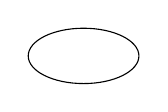
\begin{tikzpicture}
  \draw (0,0) ellipse (20pt and 10pt);
\end{tikzpicture}

\subsection{Rectangle path}
\label{sec:rectangle-path}

\begin{lstlisting}
\filldraw [gray] (0,0) circle (2pt);
\filldraw [gray] (0.5,0.5) circle (2pt);
  \draw (0,0) rectangle (0.5,0.5);
\end{lstlisting}


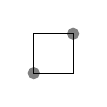
\begin{tikzpicture}
  \filldraw [gray] (0,0) circle (2pt);
  \filldraw [gray] (0.5,0.5) circle (2pt);
  \draw (0,0) rectangle (0.5,0.5);
\end{tikzpicture}

\subsection{Grid path}
\label{sec:grid-path}

\begin{lstlisting}
  \filldraw [gray] (-1.4,-1.4) circle (2pt);
  \filldraw [gray] (1.4,1.4) circle (2pt);

  \draw[step=.5cm,gray,very thin] (-1.4,-1.4) grid (1.4,1.4);
\end{lstlisting}

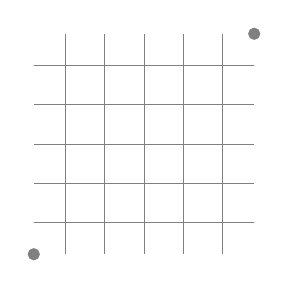
\begin{tikzpicture}
  \filldraw [gray] (-1.4,-1.4) circle (2pt);
  \filldraw [gray] (1.4,1.4) circle (2pt);

  \draw[step=.5cm,gray,very thin] (-1.4,-1.4) grid (1.4,1.4);
\end{tikzpicture}


\subsection{Arc path}
\label{sec:arc-path}

\begin{lstlisting}
  \filldraw [gray] (0,0) circle (2pt);
  \draw (0mm,0mm) arc (0:30:3cm);
  % (center) arc (angle1:angle2:radius)
  % an arc from angle1 to angle2 on a circle of radius

\end{lstlisting}

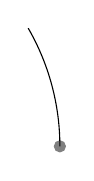
\begin{tikzpicture}
  \filldraw [gray] (0,0) circle (2pt);

  \draw (0mm,0mm) arc (0:30:3cm);
  % (center) arc (angle1:angle2:radius)
  % an arc from angle1 to angle2 on a circle of radius
\end{tikzpicture}



\subsection{Clipping a path}
\label{sec:clipping-path}
\begin{lstlisting}
  \draw[step=.5cm,gray,very thin] (-1.4,-1.4) grid (1.4,1.4);
  \draw (-1.5,0) -- (1.5,0);
  \draw (0,-1.5) -- (0,1.5);
  \draw (0,0) circle (1cm);
  \draw (3mm,0mm) arc (0:30:3mm);  

\end{lstlisting}

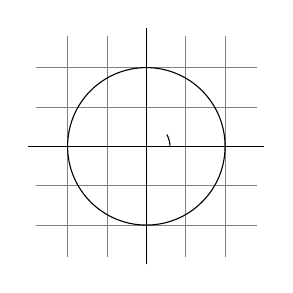
\begin{tikzpicture}
  \draw[step=.5cm,gray,very thin] (-1.4,-1.4) grid (1.4,1.4);
  \draw (-1.5,0) -- (1.5,0);
  \draw (0,-1.5) -- (0,1.5);
  \draw (0,0) circle (1cm);
  \draw (3mm,0mm) arc (0:30:3mm);  
\end{tikzpicture}

\begin{lstlisting}
  \clip (-0.1,-0.2) rectangle (1.1,0.75);
  \draw[step=.5cm,gray,very thin] (-1.4,-1.4) grid (1.4,1.4);
  \draw (-1.5,0) -- (1.5,0);
  \draw (0,-1.5) -- (0,1.5);
  \draw (0,0) circle (1cm);
  \draw (3mm,0mm) arc (0:30:3mm);  

\end{lstlisting}

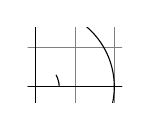
\begin{tikzpicture}
  \clip (-0.1,-0.2) rectangle (1.1,0.75);
  \draw[step=.5cm,gray,very thin] (-1.4,-1.4) grid (1.4,1.4);
  \draw (-1.5,0) -- (1.5,0);
  \draw (0,-1.5) -- (0,1.5);
  \draw (0,0) circle (1cm);
  \draw (3mm,0mm) arc (0:30:3mm);  
\end{tikzpicture}

In reality, \keyword{\textbackslash{}draw} is just a shorthand for \keyword{\textbackslash{}path[draw]} and \keyword{\textbackslash{}clip} is a shorthand for \keyword{\textbackslash{}path[clip]} and you could also say \keyword{\textbackslash{}path[draw,clip]}.



\subsection{Filling}
\label{sec:filling}

\begin{lstlisting}
\fill[green!20!white] (0,0) -- (3cm,0cm) arc (0:30:3cm) -- cycle;
\end{lstlisting}


\begin{tikzpicture}
  \fill[green!20!white] (0,0) -- (3cm,0cm) arc (0:30:3cm) -- cycle;
\end{tikzpicture}


The \keyword{--cycle} causes the current path to be closed.


You can also fill and draw a path at the same time using the \keyword{\textbackslash{}filldraw} command.


\subsection{Shading}
\label{sec:shading}

\keyword{\textbackslash{}shade} and \keyword{\textbackslash{}shadedraw} are used for shading and drawing at the same time.

\begin{lstlisting}
  \shade (0,0) rectangle (2,1);
  \shade[top color=yellow,bottom color=black] (3,0) rectangle +(2,1);
  \shade[left color=yellow,right color=black] (6,0) rectangle +(2,1); % relative coordinate
  \shadedraw[inner color=yellow,outer color=black,draw=yellow] (9,0) rectangle +(2,1);
  \shade[ball color=green] (12,.5) circle (.5cm);
\end{lstlisting}


\begin{tikzpicture}
  \shade (0,0) rectangle (2,1);
  \shade[top color=yellow,bottom color=black] (3,0) rectangle +(2,1);
  \shade[left color=yellow,right color=black] (6,0) rectangle +(2,1);
  \shadedraw[inner color=yellow,outer color=black,draw=yellow] (9,0) rectangle +(2,1);
  \shade[ball color=green] (12,.5) circle (.5cm);
\end{tikzpicture}

The default shading is a smooth transition from gray to white. To specify different colors, you can use options.



\subsection{Specifying coordinates}
\label{sec:spec-coord}

\begin{itemize}
\item If you leave out the unites, the default are set to cm and for angle to degree.
\item \keyword{+} means a relative coordinate from the previous specified position and \keyword{++} means a relative coordinate from the previous specified position, making this the new specified position.
\item You can use \keyword{intersection} to specify a coordinate.
\end{itemize}


\begin{lstlisting}
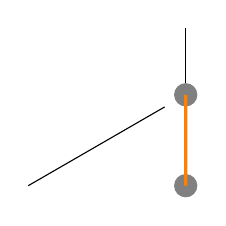
\begin{tikzpicture}[scale=2]
  \draw (1,0) -- (1,1);
  \draw (0,0) -- (30:1cm);
  \filldraw [gray] (1,0) circle (2pt);
  \filldraw [gray] (intersection of 1,0--1,1 and 0,0--30:1cm) circle (2pt);
  \draw[very thick,orange] (1,0) -- (intersection of 1,0--1,1 and 0,0--30:1cm);
\end{tikzpicture}

\end{lstlisting}

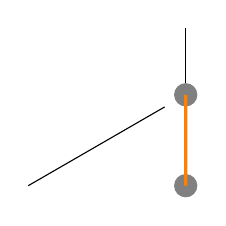
\begin{tikzpicture}[scale=2]
  \draw (1,0) -- (1,1);
  \draw (0,0) -- (30:1cm);
  \filldraw [gray] (1,0) circle (2pt);
  \filldraw [gray] (intersection of 1,0--1,1 and 0,0--30:1cm) circle (2pt);
  \draw[very thick,orange] (1,0) -- (intersection of 1,0--1,1 and 0,0--30:1cm);
\end{tikzpicture}


\subsection{Adding arrow tips}
\label{sec:adding-arrow}


\begin{lstlisting}
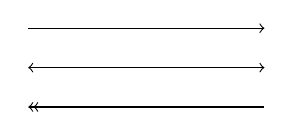
\begin{tikzpicture}
  \draw[->] (-1.5,0) -- (1.5,0);
  \draw[<->] (-1.5,-0.5) -- (1.5,-0.5);
  \draw[<<-] (-1.5,-1) -- (1.5,-1);
\end{tikzpicture}
\end{lstlisting}

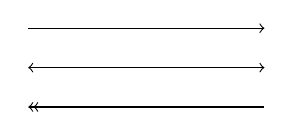
\begin{tikzpicture}
  \draw[->] (-1.5,0) -- (1.5,0);
  \draw[<->] (-1.5,-0.5) -- (1.5,-0.5);
  \draw[<<-] (-1.5,-1) -- (1.5,-1);
\end{tikzpicture}

\begin{lstlisting}
\begin{tikzpicture}[>=stealth]  % >= right arrow tip kind
  \draw[->] (-1.5,0) -- (1.5,0);
\end{tikzpicture}
\end{lstlisting}

\begin{tikzpicture}[>=stealth]  % >= right arrow tip kind
  \draw[->] (-1.5,0) -- (1.5,0);
\end{tikzpicture}



\subsection{Scoping}
\label{sec:scoping}

Scope can let you apply graphic options to a local group.

\begin{lstlisting}
\begin{tikzpicture}[ultra thick]
  \draw (0,0) -- (0,1);
  \begin{scope}[thin]
    \draw (1,0) -- (1,1);
    \draw (2,0) -- (2,1);
  \end{scope}
  \draw (3,0) -- (3,1);
\end{tikzpicture}
\end{lstlisting}

\begin{tikzpicture}[ultra thick]
  \draw (0,0) -- (0,1);
  \begin{scope}[thin]
    \draw (1,0) -- (1,1);
    \draw (2,0) -- (2,1);
  \end{scope}
  \draw (3,0) -- (3,1);
\end{tikzpicture}


\subsection{Transformations}
\label{sec:transformations}

When you specify a coordinate, TikZ applies certain transformations to the given coordinate in order to determine the finally position on the page.

\begin{lstlisting}

\begin{tikzpicture}[even odd rule,rounded corners=2pt,x=10pt,y=10pt]
  % x=10pt set the x unit to 10pt
  \filldraw (0,0)   rectangle (1,1)
  [xshift=5pt,yshift=5pt]   (0,0)   rectangle (1,1)
  [rotate=30]   (-1,-1) rectangle (2,2);

\end{tikzpicture}

\end{lstlisting}


\begin{tikzpicture}[even odd rule,rounded corners=2pt,x=10pt,y=10pt]
  % x=10pt set the x unit to 10pt
  \filldraw (0,0)   rectangle (1,1)
  [xshift=5pt,yshift=5pt]   (0,0)   rectangle (1,1)
  [rotate=30]   (-1,-1) rectangle (2,2);

\end{tikzpicture}

Options to do transformations:
\begin{itemize}
\item \keyword{xshift} and \keyword{yshift}
\item \lstinline|shift={(1,0)}| for shifting to a given point
\item \keyword{rotate} for rotating by a certain angle
\item \keyword{rotate around} for rotating around a given point
\item \keyword{scale} for scaling by a certain factor
\item \keyword{xscale} and \keyword{yscale} (\keyword{xscale=-1} is a flip)
\item \keyword{xslant} and \keyword{yslant} for slanting
\end{itemize}



\subsection{For-loops}
\label{sec:loops}
PGF introduces a command called \keyword{\textbackslash{}foreach}.
The general syntax is
\begin{lstlisting}
\foreach variable in {list of values} command
\end{lstlisting}

\begin{lstlisting}
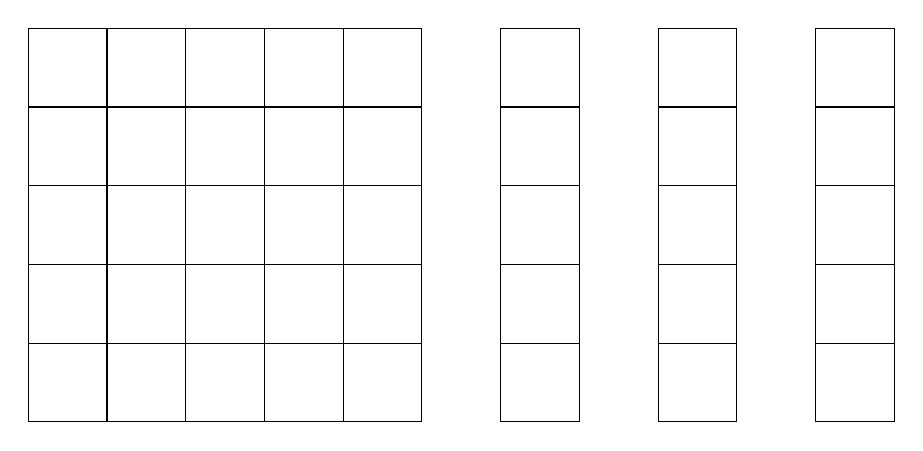
\begin{tikzpicture}
  \foreach \x in {1,2,...,5,7,9,...,12}
    \foreach \y in {1,...,5}
    {
      \draw (\x,\y) +(-.5,-.5) rectangle ++(.5,.5);
    }
\end{tikzpicture}

\end{lstlisting}

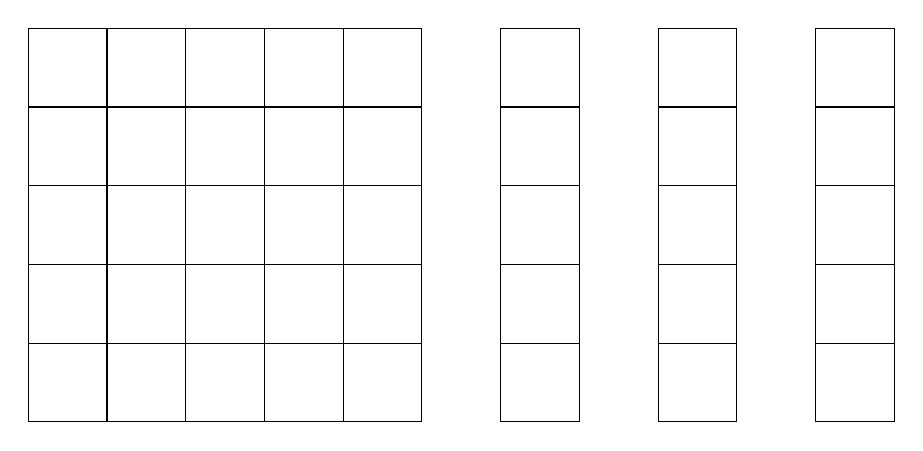
\begin{tikzpicture}
  \foreach \x in {1,2,...,5,7,9,...,12}
    \foreach \y in {1,...,5}
    {
      \draw (\x,\y) +(-.5,-.5) rectangle ++(.5,.5);
    }
\end{tikzpicture}

If you provide two numbers before the \keyword{...}, the \keyword{\textbackslash{}foreach} statement will use their difference for the stepping.

\subsection{Adding text}
\label{sec:adding-text}

\begin{lstlisting}
\begin{tikzpicture}
  \draw (0,0) -- node[above=1pt] {above=1pt} (3,0)
  (0,-1) -- node[anchor=north] {anchor=north} (3,-1);
  \draw (0,-3) .. controls (6,-2) and (9,-2) ..
  node[near start,sloped,above] {near start}
  node {midway}
  node[very near end,sloped,below] {very near end} (12,-3);
\end{tikzpicture}
\end{lstlisting}


\begin{tikzpicture}
  \draw (0,0) -- node[above=1pt] {above=1pt} (3,0)
  (0,-1) -- node[anchor=north] {anchor=north} (3,-1);
  \draw (0,-3) .. controls (6,-2) and (9,-2) ..
  node[near start,sloped,above] {near start}
  node {midway}
  node[very near end,sloped,below] {very near end} (12,-3);
\end{tikzpicture}

When TikZ is constructing a path and encounters the keyword \keyword{node} in the middle of a path, it reads a ``node specification''.
The keyword \keyword{node} is typically followed by some options and then some text between curly braces.
This text is put inside a normal TEX box.
All nodes are drawn only after the path has been completely drawn.
You can determine the direction to the position with the \keyword{anchor} option.
And there are simplified writing for the \keyword{anchor} option.
\keyword{below} does the same as \keyword{anchor=south east}.
You can also position labels on curves and, by adding the \keyword{sloped} option, have them rotated such that they match the line’s slope.


\section{Examples}
\label{sec:examples}


\message{ !name(latex.tex) !offset(-426) }
